\documentclass[journal, a4paper]{IEEEtran}


\usepackage{graphicx}   
\begin{document}

% Define document title and author

\font\myfont=cmr12 at 16pt

	\title{\myfont  Speed of Light Measurements with a Helium-Neon Laser }
	\author{Litawn Gan
	\thanks{}}
	\markboth{Physics 107. Lab 2}{}
	\maketitle
    
\begin{abstract}
We measure the speed of light $c$ using laser interferometry techniques. By varying the length of a Helium-Neon laser cavity, we obtain the frequency spacing between longitudinal modes. Based on the relationship between the speed of light and the free spectral range frequency, we deduce a value of $2.98 \pm .02 m/s$ for $c$. We analyze the limitations of this particular experiment, specifically the imprecision of the initial length measurements as well as the systematic effects of frequency pulling and pushing.
\end{abstract}

% Each section begins with a \section{title} command
\section{Introduction}

The speed of light is a universal physical constant that bridges the fundamental concepts of space and time. Its value specifies the maximum speed at which matter and information can be propagated in the universe. The precise measurement of the quantity has a storied history, as generations of theoretical and experimental physicists have devoted energy to the problem \cite{measure}  The accepted value today is 299,792,458 m/s, with the modern meter defined to satisfy this relation \cite{speed}.

Measuring the speed of light can be accomplished with a Helium-Neon laser. While lasers are designed to emit coherent light, a given laser cavity has several distinct longitudinal modes associated with it. Light at certain  modal frequencies constructively interfere when reflecting off the cavity's reflecting surfaces, while all other frequencies are suppressed by destructive interference.  When light from multiple modes is projected onto a photodiode, the photocurrent oscillates at the beat frequency, the frequency difference between adjacent modes.

\begin{figure}[!hbt]
		% Center the figure.
		\begin{center}
		% Include the eps file, scale it such that it's width equals the column width. You can also put width=8cm for example...
		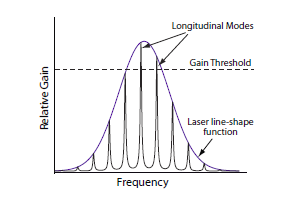
\includegraphics[width=\columnwidth]{longitudinal_modes.png}
		% Create a subtitle for the figure.
		\caption{The evenly spaced longitudinal modes of a typical laser. \cite{beat}  As can be seen, laser light must be pass a certain gain threshold in order for multiple modes to be present. Two longitudinal modes are outputted in the laser above.}
		
		\label{fig:tf_plot}
		\end{center}
	\end{figure}



This beat frequency is the free spectral range of a laser and is functionally related with the speed of light $c$. It is the round-trip time necessary for a beam of light to travel through a resonator of length $L$ and group index of refraction $n$.
$$ \nu_{FSR} =  \frac{c}{2nL} $$
Using this  relation, we can estimate the speed of light by measuring the free spectral range at different cavity lengths.

There are two primary drawbacks to this approach: the imprecision of the initial cavity length and index of refraction measurements. We elaborate on the expected magnitude of these effects and how to circumvent these problems in future experiments.

\section{Experimental Methods}

The central apparatus in the experiment is a 10 mW Helium-Neon laser designed to project photons with wavelengths of 632.8 nm. The laser cavity consists of a mirror on one end and a Brewster window on the opposite end. The Brewster window filters out polarizations orthogonal to the Brewster plane, ensuring that the measured beat frequency will in fact be the free spectral range frequency.

Laser alignment is accomplished on an optical table with the HeNe discharge tube, irises, high-reflector mirrors, and output-coupler mirrors. Our experimental data was produced with a laser power output of .7 mW, measured at the input of the photodiode. The irises were placed in the laser cavity to restrict gain from the center of the optical axis, isolating the $TEM_{00}$ mode. Isolating one transverse mode is necessary because higher-order modes have different beat frequencies that can complicate the measurement.\cite{beat}

The output of the laser is directed into a fast photodiode which communicates with an RF frequency spectrum analyzer.  For every iteration of length, the location of the beat frequency is noted. We fit the experimental data with the functional relationship between the speed of light, resonator length, and free spectral range.

\section{Uncertainty Analysis and Results}

Figure 2 represents measurement data for 27 cavity lengths.  The uncertainty in our initial cavity length $ L $  was $\pm .5$ cm, determined by uncertain locations of the ends of the laser cavity. The uncertainty in our length increment $\Delta L$ was minuscule in comparison, $\pm .01 $ cm, thanks to the high precision of the micrometer.

Unlike $L$ and $\Delta L$, uncertainty in the beat frequency $\nu$ was not dominated by measurement errors, but rather frequency pushing and pulling. Frequency pulling occurs when the index of refraction in the laser cavity effects each transverse mode differently (it is lower for frequencies beneath the resonance transition and higher for frequencies above it)\cite{beat}. It effectively decreases the beat frequency between modes and the free spectral range as modes are pulled towards the center of the gain curve. Fluctuations from this effect are about .03 to .04 MHz\cite{pulling}. A way to address frequency pulling in future experiments is to use a Fabry-Perot interferometer to equalize the intensities of the laser's longitudinal modes. This minimizes the refractive index difference between longitudinal modes, and reduces the pulling effect.

Frequency pushing, on the other hand, is related with the total gain in the laser cavity. In general, as gain in the laser cavity is increased, the beat frequency measured on the photodiode increases \cite{beat}. This systematic error manifests when variations in the voltage from the power supply effect the behavior of the oscillator. Fluctuations due to this effect are about .01 MHz for small $\pm 10 \%$ variations in total laser amplitude.  Like frequency pulling, frequency pushing can be minimized with the use of a  Fabry-Perot interferometer to ensure that the two longitudinal modes measured are at the same total amplitude.

Our best estimate of the magnitude of frequency pulling and pushing effects, $\pm .05$ MHz, masks out the measurement uncertainty of $\pm .001$ MHz from the spectrum analyzer. 
\begin{figure}[!hbt]
		% Center the figure.
		\begin{center}
		% Include the eps file, scale it such that it's width equals the column width. You can also put width=8cm for example...
		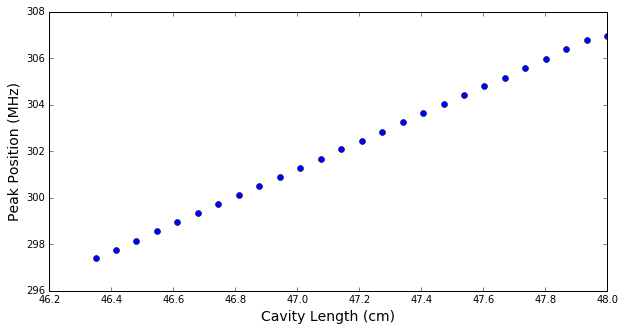
\includegraphics[width=\columnwidth]{figure_2.png}
		% Create a subtitle for the figure.
		\caption{The frequency locations for 26 different cavity lengths. Error bars are too small to display on this scale; the measurement uncertainty in frequency is about $.001 $ MHz, dictated by the scale of the spectrum analyzer.}
		
		\label{fig:tf_plot}
		\end{center}
	\end{figure}
    
Another source of systematic error originates from the environment of the laser. Minor issues with signal consistency were observed due to the dust and air particles. While the effect was small in still air, small breezes would perturb our data significantly. This uncertainty affected the amplitude of our free spectral range measurements, but should have a much smaller effect on the actual frequencies measured as compared to the $\pm .05$ MHz uncertainty from frequency pushing and pulling. With no vacuum chamber, we resorted to shielding the laser beam path with makeshift covers.

\begin{figure}[!hbt]
		% Center the figure.
		\begin{center}
		% Include the eps file, scale it such that it's width equals the column width. You can also put width=8cm for example...
		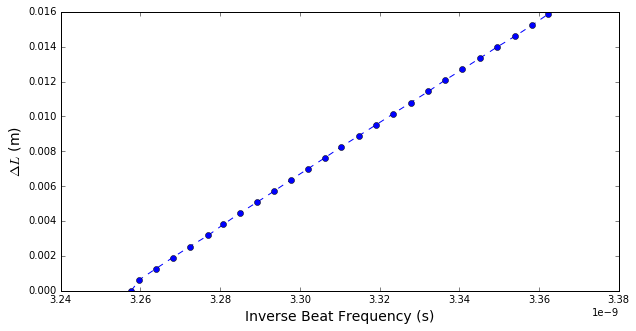
\includegraphics[width=\columnwidth]{deltaLbeat.png}
		% Create a subtitle for the figure.
		\caption{Length increments $\Delta L$ in relation to inverse beat frequency $\frac{1}{\nu_{FSR}}$ with a linear regression plotted over the data points. Error bars are too small to see at this scale. The slope of this line is $ 1.490 \pm .009 \times 10^8 m/s$  with uncertainties derived from the linear regression.}
		
		\label{fig:tf_plot}
		\end{center}
	\end{figure}
Figure 3 shows the graphed relationship between length increments $\Delta L $ and inverse beat frequency $\frac{1}{\nu_{FSR}}$.  According to the free spectral range equation, the slope of this line is $c/2n$. By modeling the index of refraction contribution as mostly from air ($n_{air} = 1.00027$), we obtain the speed of light:

$$c = 2.98 \pm .02 m/s $$
\section{Conclusion}

Two limits on precision remain after the analysis outlined in this experiment. The length of the entire laser cavity $L_{HeNe}$ and the index of refraction of the material constituting the cavity $n_{HeNe}$ are both relevant when considering higher order $TEM_{ij}$ modes and the pattern of beat frequencies produced. The allowed frequencies for higher order modes can be summarized in the following equation \cite{beat}: 

$$f_{Nij} = \frac{c}{2L} [N + \frac{1}{\pi}(i + j + 1 )cos^{-1}(\sqrt{g_{1}g_{2}})]$$
where $g_{1}g_{2}$ represents the resonator's stability. While this particular experiment utilized the $TEM_{00}$ modes, and could therefore relegate the $L_{HeNe}$ and $n_{HeNe}$ terms to the y-intercept of the $\Delta L$ versus $\frac{1}{\nu_{FSR}}$ graph,  precise measurements of these unknown parameters would be a natural evolution of a further exploration into the speed of light. 




\begin{thebibliography}{5}


	\bibitem{measure} % Conference paper
	K. M. Evenson, J.S. Wells, F.R. Peterson, B.L. Danielson \& G.W. Day, {\em Speed of Light from Direct Frequency and Wavelength Measurements of the Methane-Stabilized Laser.} Phys. Rev. Lett. 29, 1346 – Published 6 November 1972.
    
    \bibitem{modes}
    Dean L. Farnham, Robert S. Van Dyck, Jr., and Paul B. {\em Determination of the Electron's Atomic Mass and the Proton/Electron Mass Ratio via Penning Trap Mass Spectroscopy.} Schwinberg
	Phys. Rev. Lett. 75, 3598
    
    \bibitem{beat} % Transaction paper
	Daniel J. D'Orazio et. al, “Measuring the speed of light using beating longitudinal modes in an open-cavity HeNe laser” Appl. Opt. 3(2), 267–275 (1964).
    
	\bibitem{speed} % 
    NIST Reference on Constants, Units, and Uncertainties, 		      																	 http://physics.nist.gov/cuu/Units/meter.html.
    
    \bibitem{pulling} %
    A. M. Lindberg, Mode frequency pulling in He-Ne
    Lasers," Am. J. Phys. 67, 350-353 (1999).

\end{thebibliography}

	
    

\end{document}
